% ============================================================================
% AD7031 Week 2 -- LECTURE NOTE
%
% Section 0: prerequisites (function, R^n, vector, matrix, quadratic form).
% Sections 1-5: gentle optimization / LP / convexity / QP review.
% Section 6 (convexity-preserving operations) converts OUU Lecture 1, pp. 2-3.
% Section 7 (probability review) covers OUU Lecture 3, pp. 1-2 (top), taught in
% engineering-probability notation (X, f(x)): random variable, PMF, PDF, 1D and
% 2D examples, independence, covariance, linear combinations; it ends with a
% map to the course's notation (tilde xi, P).
% Section 8 is the running example -- Markowitz, with the coding session's data
% (notebooks/week03_markowitz.ipynb, demos/markowitz_portfolio.py).
% Both follow the handwritten notes' Def/list structure; duality gets its own
% session next week. Self-contained on purpose -- no \input{preamble} -- so it
% compiles wherever it is dropped.
% ============================================================================
\documentclass[10pt]{article}

\usepackage[a4paper, margin=1.9cm]{geometry}
\usepackage{amsmath, amssymb}
\usepackage[dvipsnames]{xcolor}
\usepackage{graphicx}
\usepackage{array}
\usepackage{tikz}
\usepackage[hidelinks]{hyperref}

\definecolor{ruleink}{RGB}{18, 68, 140}
\definecolor{demoink}{RGB}{140, 82, 20}
\definecolor{keyink}{RGB}{20, 90, 20}
\definecolor{watchink}{RGB}{86, 60, 140}
\definecolor{punchink}{RGB}{170, 30, 60}
\definecolor{lineA}{RGB}{44, 110, 176}
\definecolor{lineB}{RGB}{168, 96, 32}
\definecolor{lineC}{RGB}{78, 62, 140}

\setlength{\parindent}{0pt}
\pagestyle{empty}

% tighter spacing around centered displays
\AtBeginDocument{%
  \abovedisplayskip=7pt plus 2pt
  \belowdisplayskip=7pt plus 2pt
  \abovedisplayshortskip=4pt
  \belowdisplayshortskip=4pt}

% ---- one section -----------------------------------------------------------
\newcommand{\beat}[2]{%   number, title
  \par\bigskip\vspace{4pt}
  {\color{ruleink}\rule{\textwidth}{1pt}}\par\nobreak\vspace{4pt}
  {\large\bfseries #1.\; #2}\par\nobreak\vspace{6pt}}

% ---- board content ---------------------------------------------------------
\newenvironment{board}{%
  \par\vspace{4pt}
  \begingroup\leftskip=1.3em\relax\parskip=2pt\relax}{%
  \par\endgroup\vspace{4pt}}

% ---- highlights ------------------------------------------------------------
% ---- short rule used to draw a row vector inside a matrix ------------------
\newcommand{\rowline}{\rule[0.55ex]{1.15em}{0.4pt}}

% ---- hanging bullet (wrapped lines stay indented) --------------------------
\newcommand{\bul}{\hangindent=2.6em\hangafter=1\hspace{1.2em}\textbullet\ \ignorespaces}

\newcommand{\demo}[2]{\par{\color{demoink}\small\textbf{demo}\quad\texttt{#1} --- #2}\par}
\newcommand{\watch}[1]{\par{\color{watchink}\small\textbf{watch}\quad #1}\par}
\newcommand{\key}[1]{\par\vspace{1pt}{\color{keyink}\small\textbf{KEY}\quad\textbf{#1}}\par}
\newcommand{\takeaway}[1]{%
  \par\vspace{6pt}\noindent
  {\color{punchink}\rule{2pt}{10pt}}\;{\color{punchink}\small\textbf{takeaway}\quad\textbf{#1}}\par\vspace{2pt}}

\begin{document}

{\Large\bfseries Week 2 --- Convexity, LP, and Probability: the Two Reviews}\\[2pt]
{\small AD7031 Optimization Under Uncertainty \quad\textbullet\quad Instructor: Prof.\ H.\ Park \quad\textbullet\quad Sep 5, 2026}

% ---------------------------------------------------------------- 0
\beat{0}{Warm-up: functions, vectors, matrices}
\begin{board}
three objects carry the whole course: a \emph{function}, a \emph{vector}, a \emph{matrix}.
\vspace{8pt}

\textbf{Function} \quad $f : A \to B$ assigns to each input $x \in A$ exactly one output $f(x) \in B$.
\ \ $A$ = domain, \ $B$ = codomain.
\vspace{4pt}

\bul $f : \mathbb{R} \to \mathbb{R}$ \quad one number in, one number out.
      \ graph $= \{(x, f(x))\}$ --- a curve in the plane
\vspace{3pt}

\bul $f : \mathbb{R}^2 \to \mathbb{R}$ \quad two numbers in, one number out.
      \ graph --- a surface in 3D; \ level set $\{x : f(x) = c\}$ --- a curve in the plane
\vspace{3pt}

\bul $f : \mathbb{R}^n \to \mathbb{R}$ \quad an objective is always of this shape: it must return a
      \emph{single} number, otherwise two decisions cannot be compared.
\vspace{6pt}

\begin{center}
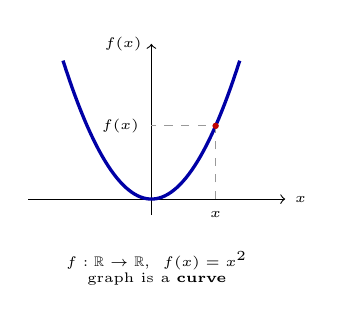
\begin{tikzpicture}[scale=0.68, font=\tiny]
  \draw[->] (-2.3,0) -- (2.5,0) node[right] {$x$};
  \draw[->] (0,-0.3) -- (0,2.9) node[left] {$f(x)$};
  \draw[very thick, blue!65!black, domain=-1.65:1.65, samples=60] plot (\x, {0.95*\x*\x});
  \draw[dashed, gray!80] (1.2,0) -- (1.2,1.368) -- (0,1.368);
  \fill[red!75!black] (1.2,1.368) circle (1.7pt);
  \node[below] at (1.2,-0.05) {$x$};
  \node[left] at (-0.05,1.368) {$f(x)$};
  \node[align=center] at (0.1,-1.3) {$f : \mathbb{R} \to \mathbb{R}$, \ $f(x) = x^2$\\ graph is a \textbf{curve}};
\end{tikzpicture}
\hspace{7mm}
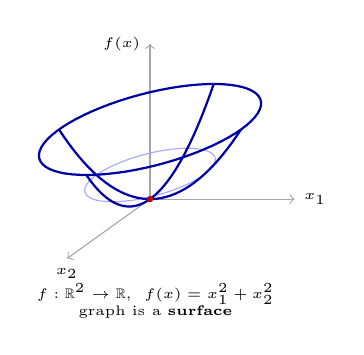
\begin{tikzpicture}[scale=0.68, font=\tiny]
  \draw[->, gray!70] (0,0) -- (2.7,0) node[right, black] {$x_1$};
  \draw[->, gray!70] (0,0) -- (-1.55,-1.11) node[below, black] {$x_2$};
  \draw[->, gray!70] (0,0) -- (0,2.9) node[left, black] {$f(x)$};
  \draw[blue!35!white, domain=0:360, samples=60]
        plot ({1.0*cos(\x) - 0.7*sin(\x)}, {-0.5*sin(\x) + 0.45});
  \draw[blue!65!black, thick, domain=0:360, samples=70]
        plot ({1.7*cos(\x) - 1.19*sin(\x)}, {-0.85*sin(\x) + 1.3});
  \draw[blue!65!black, thick, domain=-1.7:1.7, samples=40] plot (\x, {0.45*\x*\x});
  \draw[blue!65!black, thick, domain=-1.7:1.7, samples=40]
        plot ({-0.7*\x}, {-0.5*\x + 0.45*\x*\x});
  \fill[red!75!black] (0,0) circle (1.7pt);
  \node[align=center] at (0.1,-1.9) {$f : \mathbb{R}^2 \to \mathbb{R}$, \ $f(x) = x_1^2 + x_2^2$\\ graph is a \textbf{surface}};
\end{tikzpicture}
\hspace{7mm}
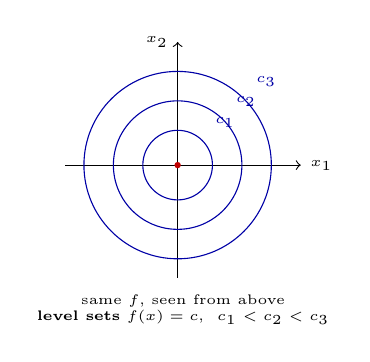
\begin{tikzpicture}[scale=0.68, font=\tiny]
  \draw[->] (-2.1,0) -- (2.3,0) node[right] {$x_1$};
  \draw[->] (0,-2.1) -- (0,2.3) node[left] {$x_2$};
  \draw[blue!65!black] (0,0) circle (0.65);
  \draw[blue!65!black] (0,0) circle (1.2);
  \draw[blue!65!black] (0,0) circle (1.75);
  \fill[red!75!black] (0,0) circle (1.7pt);
  \node[blue!65!black, anchor=south west] at (0.52,0.52) {$c_1$};
  \node[blue!65!black, anchor=south west] at (0.91,0.91) {$c_2$};
  \node[blue!65!black, anchor=south west] at (1.29,1.29) {$c_3$};
  \node[align=center] at (0.1,-2.7) {same $f$, seen from above\\ \textbf{level sets} $f(x) = c$, \ $c_1 < c_2 < c_3$};
\end{tikzpicture}
\end{center}
\vspace{10pt}

\textbf{Real space} \quad $\mathbb{R}$ = all real numbers --- a line. \quad
$\mathbb{R}^n$ = lists of $n$ real numbers:
\vspace{3pt}

\quad $x = (x_1, x_2, \dots, x_n)$, \quad $x_i \in \mathbb{R}$
\vspace{3pt}

\quad $n = 1$: line, \quad $n = 2$: plane, \quad $n = 3$: space, \quad $n \ge 4$: same algebra, no picture
\vspace{3pt}

\quad ``$x \in \mathbb{R}^n$'' \ = \ one list of $n$ numbers \ = \ one point \ = \ one arrow from the origin \ = \ \textbf{one decision}
\vspace{5pt}

\begin{center}
\begin{tikzpicture}[scale=0.68, font=\tiny]
  \draw[->] (-2.2,0) -- (2.4,0) node[right] {$\mathbb{R}$};
  \foreach \t in {-2,-1,0,1,2} \draw (\t,0.09) -- (\t,-0.09) node[below] {$\t$};
  \fill[red!75!black] (1.5,0) circle (1.7pt);
  \node[above, red!75!black] at (1.5,0.08) {$x = 1.5$};
  \node at (0,-1.15) {$n = 1$};
\end{tikzpicture}
\hspace{9mm}
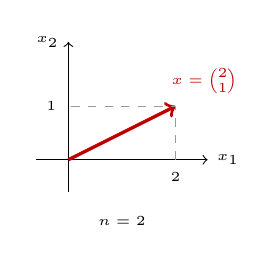
\begin{tikzpicture}[scale=0.68, font=\tiny]
  \draw[->] (-0.6,0) -- (2.6,0) node[right] {$x_1$};
  \draw[->] (0,-0.6) -- (0,2.2) node[left] {$x_2$};
  \draw[->, very thick, red!75!black] (0,0) -- (2.0,1.0);
  \draw[dashed, gray!80] (2.0,0) -- (2.0,1.0) -- (0,1.0);
  \node[below] at (2.0,-0.05) {$2$}; \node[left] at (-0.05,1.0) {$1$};
  \node[anchor=south west, red!75!black] at (1.75,1.05) {$x = \binom{2}{1}$};
  \node at (1.0,-1.15) {$n = 2$};
\end{tikzpicture}
\hspace{9mm}
\begin{tikzpicture}[scale=0.68, font=\tiny]
  \draw[->] (0,0) -- (2.3,0) node[right] {$x_1$};
  \draw[->] (0,0) -- (-1.25,-0.9) node[below] {$x_2$};
  \draw[->] (0,0) -- (0,2.1) node[left] {$x_3$};
  \draw[dashed, gray!80] (1.0,0.85) -- (1.0,0.0) -- (0,0);
  \draw[->, very thick, red!75!black] (0,0) -- (1.0,0.85);
  \fill[red!75!black] (1.0,0.85) circle (1.7pt);
  \node at (0.4,-1.35) {$n = 3$};
\end{tikzpicture}
\end{center}
\vspace{10pt}

\textbf{Vector} \quad by convention a \emph{column}: \ $x \in \mathbb{R}^n$ is $n \times 1$. \
transpose $x^{\top}$ is the row, $1 \times n$.
\vspace{4pt}

\bul \textbf{inner product} of $c, x \in \mathbb{R}^n$: \quad$c^{\top}x = c_1x_1 + \cdots + c_nx_n = \sum_{i=1}^{n} c_i x_i$
\vspace{3pt}

\qquad as a function: \quad $f(x) = c^{\top}x$, \quad $f : \mathbb{R}^n \to \mathbb{R}$ \quad --- fix $c$, feed it $x$, get one number
\vspace{2pt}

\qquad Section 3's objective: $c$ = prices, $x$ = amounts, $f(x) = c^{\top}x$ = value of the cargo
\vspace{5pt}

\bul \textbf{2-norm} of $x \in \mathbb{R}^n$: \quad$\|x\|_2 = \sqrt{x^{\top}x} = \sqrt{x_1^2 + \cdots + x_n^2}$
\vspace{3pt}

\qquad as a function: \quad $f(x) = \|x\|_2$, \quad $f : \mathbb{R}^n \to \mathbb{R}$ \quad --- again one number out
\vspace{10pt}

\textbf{Matrix} \quad a matrix is a \emph{stack of row vectors}:
\[
A = \begin{pmatrix}
  \rowline\; a_1^{\top} \;\rowline \\[3pt]
  \rowline\; a_2^{\top} \;\rowline \\[1pt]
  \vdots \\[1pt]
  \rowline\; a_m^{\top} \;\rowline
\end{pmatrix} \in \mathbb{R}^{m \times n},
\qquad a_1, a_2, \dots, a_m \in \mathbb{R}^n
\]
$m$ = number of rows, \quad $n$ = length of each row.
\vspace{6pt}

\textbf{Example} \quad $m = 3$, $n = 4$:
\[
A = \begin{pmatrix}
 1 & 3 & 0 & 2 \\
 3 & 1 & 4 & 0 \\
 0 & 2 & 1 & 5
\end{pmatrix} \in \mathbb{R}^{3 \times 4},
\qquad
a_1 = \begin{pmatrix} 1 \\ 3 \\ 0 \\ 2 \end{pmatrix}, \quad
a_2 = \begin{pmatrix} 3 \\ 1 \\ 4 \\ 0 \end{pmatrix}, \quad
a_3 = \begin{pmatrix} 0 \\ 2 \\ 1 \\ 5 \end{pmatrix} \in \mathbb{R}^4
\]
\vspace{2pt}

\bul \textbf{matrix $\times$ vector:} \ for $x \in \mathbb{R}^n$, \ $Ax \in \mathbb{R}^m$ \ with \
$(Ax)_i = a_i^{\top}x$ \quad --- one inner product per row
\vspace{2pt}

\[
x = \begin{pmatrix} 1 \\ 2 \\ 1 \\ 0 \end{pmatrix} \in \mathbb{R}^4:
\qquad
Ax = \begin{pmatrix} a_1^{\top}x \\[2pt] a_2^{\top}x \\[2pt] a_3^{\top}x \end{pmatrix}
   = \begin{pmatrix} 1 + 6 + 0 + 0 \\ 3 + 2 + 4 + 0 \\ 0 + 4 + 1 + 0 \end{pmatrix}
   = \begin{pmatrix} 7 \\ 9 \\ 5 \end{pmatrix} \in \mathbb{R}^3
\]

\qquad as a function: \quad $f(x) = Ax$, \quad $f : \mathbb{R}^4 \to \mathbb{R}^3$
\vspace{2pt}

\qquad\qquad --- takes a $4$-dimensional vector, returns a $3$-dimensional vector; not a single number (a \emph{scalar})
\vspace{2pt}

\qquad\qquad in general \ $f(x) = Ax$, \ $f : \mathbb{R}^n \to \mathbb{R}^m$
\vspace{6pt}

\bul \textbf{identity matrix} $I \in \mathbb{R}^{n \times n}$: \ $1$'s on the diagonal, $0$'s elsewhere.
\ its rows are $e_1^{\top}, \dots, e_n^{\top}$
\vspace{2pt}

\qquad $I = \begin{pmatrix} 1 & 0 & 0 \\ 0 & 1 & 0 \\ 0 & 0 & 1 \end{pmatrix} \in \mathbb{R}^{3 \times 3}$,
\qquad $(Ix)_i = e_i^{\top}x = x_i$, \ so \ $Ix = x$ \ for every $x$
\vspace{6pt}

\bul \textbf{transpose} $A^{\top} \in \mathbb{R}^{n \times m}$: rows become columns. \
$A$ is \textbf{symmetric} if $A = A^{\top}$ (so $m = n$)
\vspace{10pt}

\textbf{Quadratic function}
\vspace{4pt}

\bul one variable: \ $f(x) = px^2 + qx + r$ \quad --- a parabola; opens upward iff $p \ge 0$
\vspace{4pt}

\bul $n$ variables: \ $f(x) = x^{\top}Qx + q^{\top}x + r$, \ $Q \in \mathbb{R}^{n \times n}$ symmetric
      \quad --- still $\mathbb{R}^n \to \mathbb{R}$, one number out
\vspace{4pt}

\qquad $n = 2$: \quad $x^{\top}Qx
  = \begin{pmatrix} x_1 & x_2 \end{pmatrix}
    \begin{pmatrix} Q_{11} & Q_{12} \\ Q_{12} & Q_{22} \end{pmatrix}
    \begin{pmatrix} x_1 \\ x_2 \end{pmatrix}
  = Q_{11}x_1^2 + 2Q_{12}x_1x_2 + Q_{22}x_2^2$
\vspace{4pt}

\qquad $Q = I$: \ $x^{\top}x = x_1^2 + x_2^2$ --- the round bowl drawn above.
\ ``opens upward'' becomes $Q \succeq 0$ (Sections 5, 6).
\end{board}

% ---------------------------------------------------------------- 1
\beat{1}{General optimization problem}
\begin{board}
\[
\begin{aligned}
  \min_x\quad & f(x) \\
  \text{s.t.}\quad & x \in X
\end{aligned}
\]
\begin{tabular}{@{}r@{\;\;}l@{\qquad}l@{}}
1. & what do we control? & \textbf{decision variables} $x$\\
2. & what do we want?    & \textbf{objective function} $f$\\
3. & what limits us?     & constraints $\to$ \textbf{feasible set} $X$\\
\end{tabular}
\vspace{4pt}

$X = \{\, x \in \mathbb{R}^n \;:\; g_i(x) \le 0 \ \ \forall i \in [m] \,\}$
\vspace{2pt}

\quad \emph{in plain English:} \ $x$ belongs to the $n$-dimensional real space $\mathbb{R}^n$,
\textbf{and} it satisfies all $m$ constraints
\vspace{1pt}

\quad\qquad $g_1(x) \le 0, \quad g_2(x) \le 0, \quad \dots, \quad g_m(x) \le 0$
\vspace{3pt}

\emph{read the symbols:} \quad $\in$ = ``is in'', \quad $\forall$ = ``for all'', \quad $[m] := \{1,\dots,m\}$, \quad s.t.\ = ``subject to''
\vspace{1pt}

\quad --- so ``\,$\forall i \in [m]$\,'' packs that whole list of $m$ constraints into one stroke
\vspace{3pt}

$h(x)=0 \iff h \le 0$ \textbf{and} $-h \le 0$
\end{board}
\takeaway{how we define $f(x)$ and $X$ determines the program class. some problems are easy to solve --- but some are not.}

% ---------------------------------------------------------------- 2
\beat{2}{One problem, three languages}
\begin{board}
\begin{tabular}{@{}l|ccc@{}}
              & OR    & ML                    & control \\ \hline
decision      & $x$   & $\theta$              & $u$ \\
uncertain data& $\xi$ & [$x$ = input, $y$ = output] & state $x$ perturbed by noise $w$ \\
\end{tabular}
\vspace{3pt}

keep an eye on that $\xi$ --- \emph{uncertain data} is exactly what this course is about. it returns in Section 7.
\end{board}
\key{optimization is not a topic inside OR --- it is the shared language of OR, ML, control.}
\watch{Brunton, \emph{Optimization: A Bootcamp for Machine Learning, Inverse Problems,
and Control} --- 22 min, supplementary.\\
\url{https://www.youtube.com/watch?v=lPBPbGmw1_4}}

% ---------------------------------------------------------------- 3
\beat{3}{Linear programs --- and why they are easy}
\begin{board}
\[
\begin{aligned}
  \max_x\quad & c^{\top}x \\
  \text{s.t.}\quad & Ax \le b
\end{aligned}
\]
$c \in \mathbb{R}^n$, \quad $A \in \mathbb{R}^{m\times n}$, \quad $b \in \mathbb{R}^m$
\vspace{4pt}

row $i$: \quad $g_i(x) = a_i^{\top}x - b_i \le 0 \iff a_i^{\top}x \le b_i$
\vspace{3pt}

stack rows $\Rightarrow A$ \qquad so \quad $a_i^{\top}x \le b_i \ \forall i \iff Ax \le b$
\vspace{3pt}

in many cases variables are nonnegative ($x \ge 0$) --- encoded in $Ax \le b$ by the rows $-x_j \le 0$
\vspace{4pt}

\begin{center}
$P = \{\, x : Ax \le b \,\}$ \ is called a \textbf{polyhedron}\\[5pt]
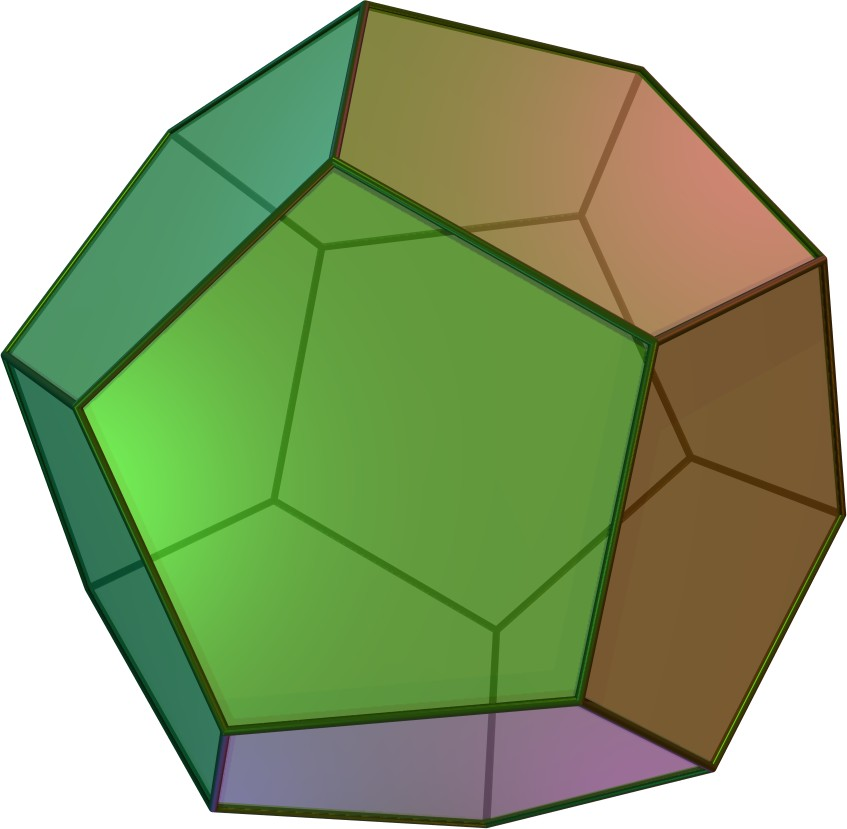
\includegraphics[height=2.6cm]{dodecahedron.jpg}\\[2pt]
{\footnotesize Polyhedron in $\mathbb{R}^3$.}
{\tiny (image: Wikimedia Commons)}
\end{center}
\vspace{2pt}

\textbf{Convexity}
\vspace{3pt}

\bul \textbf{Convex set:} \ $S \subseteq \mathbb{R}^n$ is convex if \ $\lambda x + (1-\lambda) y \in S$
      \ for all $x,y \in S$ and all $\lambda \in [0,1]$
\vspace{3pt}

\bul \textbf{Convex function:} \ $f : \mathbb{R}^n \to \mathbb{R}$ is convex if
\vspace{1pt}

\quad\qquad $f(\lambda x + (1-\lambda) y) \;\le\; \lambda f(x) + (1-\lambda) f(y)$
      \ for all $x,y \in \mathbb{R}^n$ and all $\lambda \in [0,1]$
\vspace{1pt}

\quad\qquad \emph{strictly} convex if strict for $x \ne y$, $\lambda \in (0,1)$
\vspace{3pt}

\bul \textbf{Convex problem:} \ $\min\{f(x) : x \in S\}$ with $S$ convex \emph{and} $f$ convex
\vspace{4pt}

\textbf{Prop.} \ in a convex problem, every local min is a global min.
\vspace{1pt}

\quad \emph{pf sketch:} \ if $f(y) < f(x^{\star})$, then $f(\lambda y + (1-\lambda)x^{\star})
      \le \lambda f(y) + (1-\lambda) f(x^{\star}) < f(x^{\star})$
\vspace{1pt}

\quad\qquad for all $\lambda \in (0,1]$ --- so better points sit arbitrarily close to $x^{\star}$.
\vspace{4pt}

\textbf{Examples}
\vspace{3pt}

\begin{tabular}{@{}l|l@{}}
 convex & not convex \\ \hline
 least squares $\|Ax-b\|_2^2$ over unconstrained $\mathcal{X}$ --- one bowl & neural-net training loss --- many dips \\
 linear $c^{\top}x$ over $P$ --- \textbf{our LP} & $\in \mathbb{Z}$: feasible set turns \textbf{discrete!} --- OL7014's turf \\
\end{tabular}
\end{board}
\begin{center}
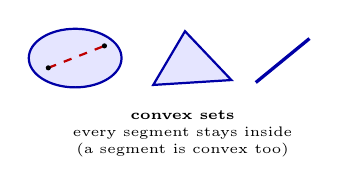
\begin{tikzpicture}[scale=0.62, font=\tiny]
  \draw[fill=blue!10, draw=blue!65!black, thick] (-2.2,0.2) ellipse (0.95 and 0.6);
  \draw[dashed, red!75!black, thick] (-2.75,0) -- (-1.6,0.45);
  \fill (-2.75,0) circle (1.5pt); \fill (-1.6,0.45) circle (1.5pt);
  \draw[fill=blue!10, draw=blue!65!black, thick] (-0.6,-0.35) -- (1.0,-0.25) -- (0.05,0.75) -- cycle;
  \draw[blue!65!black, very thick] (1.5,-0.3) -- (2.6,0.6);
  \node[align=center] at (0,-1.35) {\textbf{convex sets}\\ every segment stays inside\\ (a segment is convex too)};
\end{tikzpicture}
\hspace{6mm}
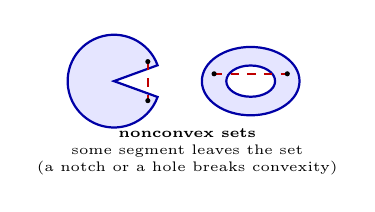
\begin{tikzpicture}[scale=0.62, font=\tiny]
  \draw[fill=blue!10, draw=blue!65!black, thick] (-1.5,0.1) -- +(20:0.95) arc (20:340:0.95) -- cycle;
  \draw[dashed, red!75!black, thick] (-0.807,0.5) -- (-0.807,-0.3);
  \fill (-0.807,0.5) circle (1.5pt); \fill (-0.807,-0.3) circle (1.5pt);
  \draw[fill=blue!10, draw=blue!65!black, thick, even odd rule]
        (1.3,0.1) ellipse (1.0 and 0.7) (1.3,0.1) ellipse (0.5 and 0.32);
  \draw[dashed, red!75!black, thick] (0.55,0.25) -- (2.05,0.25);
  \fill (0.55,0.25) circle (1.5pt); \fill (2.05,0.25) circle (1.5pt);
  \node[align=center] at (0,-1.35) {\textbf{nonconvex sets}\\ some segment leaves the set\\ (a notch or a hole breaks convexity)};
\end{tikzpicture}
\hspace{6mm}
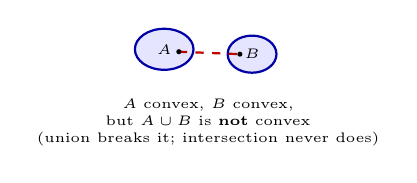
\begin{tikzpicture}[scale=0.62, font=\tiny]
  \draw[fill=blue!10, draw=blue!65!black, thick] (-0.85,0.15) ellipse (0.6 and 0.42);
  \draw[fill=blue!10, draw=blue!65!black, thick] (0.95,0.05) ellipse (0.5 and 0.38);
  \node at (-0.85,0.15) {$A$}; \node at (0.95,0.05) {$B$};
  \draw[dashed, red!75!black, thick] (-0.55,0.1) -- (0.7,0.05);
  \fill (-0.55,0.1) circle (1.5pt); \fill (0.7,0.05) circle (1.5pt);
  \node[align=center] at (0.05,-1.35) {$A$ convex, $B$ convex,\\ but $A \cup B$ is \textbf{not} convex\\ (union breaks it; intersection never does)};
\end{tikzpicture}
\end{center}
\begin{center}
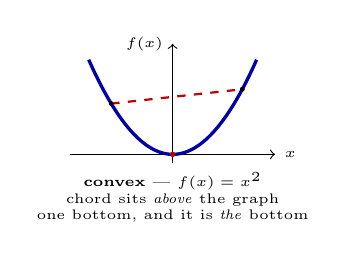
\begin{tikzpicture}[scale=0.52, font=\tiny]
  \draw[->] (-2.5,0) -- (2.5,0) node[right] {$x$};
  \draw[->] (0,-0.2) -- (0,2.7) node[left] {$f(x)$};
  \draw[very thick, blue!65!black, domain=-2.05:2.05, samples=70] plot (\x, {0.55*\x*\x});
  \draw[dashed, red!75!black, thick] (-1.5,1.24) -- (1.7,1.59);
  \fill (-1.5,1.24) circle (1.7pt); \fill (1.7,1.59) circle (1.7pt);
  \fill[red!75!black] (0,0) circle (1.9pt);
  \node[align=center] at (0,-1.05) {\textbf{convex} --- $f(x)=x^{2}$\\ chord sits \emph{above} the graph\\ one bottom, and it is \emph{the} bottom};
\end{tikzpicture}
\hspace{6mm}
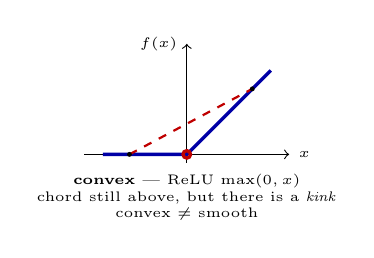
\begin{tikzpicture}[scale=0.52, font=\tiny]
  \draw[->] (-2.5,0) -- (2.5,0) node[right] {$x$};
  \draw[->] (0,-0.2) -- (0,2.7) node[left] {$f(x)$};
  \draw[very thick, blue!65!black] (-2.05,0) -- (0,0) -- (2.05,2.05);
  \draw[dashed, red!75!black, thick] (-1.4,0) -- (1.6,1.6);
  \fill (-1.4,0) circle (1.7pt); \fill (1.6,1.6) circle (1.7pt);
  \draw[red!75!black, very thick] (0,0) circle (2.6pt);
  \node[align=center] at (0,-1.05) {\textbf{convex} --- ReLU $\max(0,x)$\\ chord still above, but there is a \emph{kink}\\ convex $\ne$ smooth};
\end{tikzpicture}
\hspace{6mm}
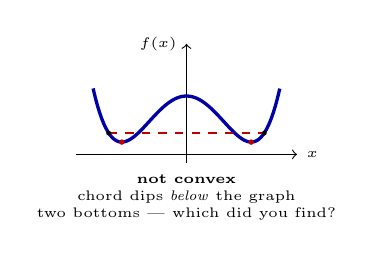
\begin{tikzpicture}[scale=0.52, font=\tiny]
  \draw[->] (-2.7,0) -- (2.7,0) node[right] {$x$};
  \draw[->] (0,-0.2) -- (0,2.7) node[left] {$f(x)$};
  \draw[very thick, blue!65!black, domain=-2.28:2.28, samples=90]
        plot (\x, {0.18*(\x*\x-2.5)*(\x*\x-2.5)+0.3});
  \draw[dashed, red!75!black, thick] (-1.9,0.52) -- (1.9,0.52);
  \fill (-1.9,0.52) circle (1.7pt); \fill (1.9,0.52) circle (1.7pt);
  \fill[red!75!black] (-1.58,0.3) circle (1.9pt); \fill[red!75!black] (1.58,0.3) circle (1.9pt);
  \node[align=center] at (0,-1.05) {\textbf{not convex}\\ chord dips \emph{below} the graph\\ two bottoms --- which did you find?};
\end{tikzpicture}
\end{center}

\begin{center}
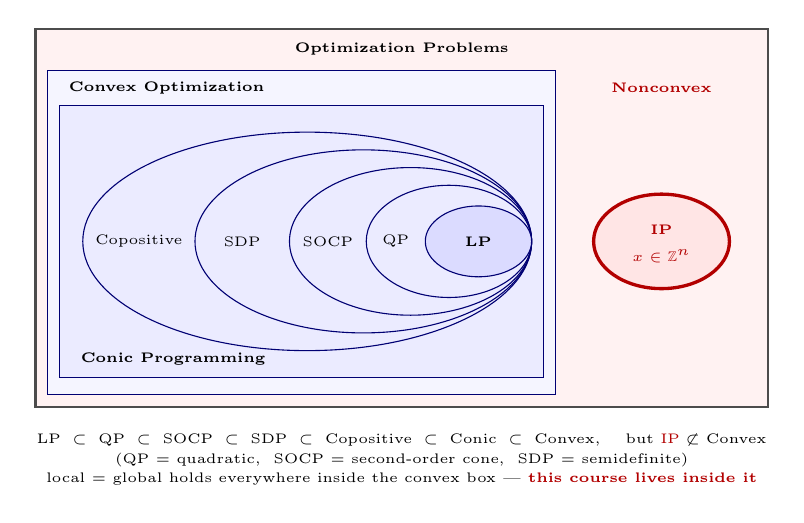
\begin{tikzpicture}[scale=0.75]
  % all optimization problems
  \draw[fill=red!5, draw=black!70, thick] (-6.2,-3.1) rectangle (6.2,3.3);
  \node[font=\tiny\bfseries] at (0, 2.95) {Optimization Problems};
  \node[font=\tiny\bfseries, color=red!70!black] at (4.4, 2.3) {Nonconvex};
  % convex optimization
  \draw[fill=blue!4, draw=blue!45!black, thin] (-6.0,-2.9) rectangle (2.6,2.6);
  \node[font=\tiny\bfseries, anchor=west] at (-5.8, 2.3) {Convex Optimization};
  % conic programming
  \draw[fill=blue!8, draw=blue!45!black, thin] (-5.8,-2.6) rectangle (2.4,2.0);
  \node[font=\tiny\bfseries, anchor=west] at (-5.6, -2.3) {Conic Programming};
  % nested classes, tangent on the right
  \draw[draw=blue!45!black, thin] (-1.6,-0.3) ellipse (3.8 and 1.85);
  \draw[draw=blue!45!black, thin] (-0.65,-0.3) ellipse (2.85 and 1.55);
  \draw[draw=blue!45!black, thin] (0.15,-0.3) ellipse (2.05 and 1.25);
  \draw[draw=blue!45!black, thin] (0.8,-0.3) ellipse (1.4 and 0.95);
  \draw[fill=blue!14, draw=blue!45!black, thin] (1.3,-0.3) ellipse (0.9 and 0.6);
  \node[font=\tiny] at (-4.45,-0.3) {Copositive};
  \node[font=\tiny] at (-2.7,-0.3) {SDP};
  \node[font=\tiny] at (-1.25,-0.3) {SOCP};
  \node[font=\tiny] at (-0.1,-0.3) {QP};
  \node[font=\tiny\bfseries] at (1.3,-0.3) {LP};
  % IP: nonconvex, for contrast
  \draw[fill=red!10, draw=red!70!black, very thick] (4.4,-0.3) ellipse (1.15 and 0.8);
  \node[font=\tiny\bfseries, color=red!70!black] at (4.4,-0.1) {IP};
  \node[font=\tiny, color=red!70!black] at (4.4,-0.55) {$x \in \mathbb{Z}^n$};
  \node[font=\tiny, align=center] at (0, -4.0)
    {$\mathrm{LP} \;\subset\; \mathrm{QP} \;\subset\; \mathrm{SOCP} \;\subset\; \mathrm{SDP} \;\subset\; \text{Copositive}
      \;\subset\; \text{Conic} \;\subset\; \text{Convex}$, \quad but ${\color{red!70!black}\mathrm{IP}} \not\subset \text{Convex}$\\[1pt]
     (QP = quadratic, \ SOCP = second-order cone, \ SDP = semidefinite)\\[1pt]
     local $=$ global holds everywhere inside the convex box --- {\color{red!70!black}\textbf{this course lives inside it}}};
\end{tikzpicture}
\end{center}
\takeaway{an LP is a convex problem: $P$ convex (intersection of half-spaces) $+$ $c^{\top}x$ linear, hence a convex function.}

% ---------------------------------------------------------------- 4
\beat{4}{First LP problem}
\begin{board}
$x$ = crates of ammo (dense), \quad $y$ = crates of rations (bulky)
\vspace{4pt}

\[
\begin{aligned}
  \max\quad & 4x + 5y \\
  \text{s.t.}\quad & x + 3y \le 10 && \text{(volume)}\\
                   & 3x + y \le 10 && \text{(weight)}\\
                   & x, y \ge 0
\end{aligned}
\]
\vspace{4pt}

\textbf{now put it in standard vector form:}
\vspace{3pt}

\quad $\mathbf{x} = \begin{pmatrix} x \\ y \end{pmatrix}$, \qquad
      $c = \begin{pmatrix} 4 \\ 5 \end{pmatrix}$, \qquad
      $A = \begin{pmatrix} 1 & 3 \\ 3 & 1 \\ -1 & 0 \\ 0 & -1 \end{pmatrix}$, \qquad
      $b = \begin{pmatrix} 10 \\ 10 \\ 0 \\ 0 \end{pmatrix}$
      \qquad (last two rows are $x, y \ge 0$)
\vspace{3pt}

\[
\begin{aligned}
  \max\quad & c^{\top}\mathbf{x} \\
  \text{s.t.}\quad & A\mathbf{x} \le b
\end{aligned}
\qquad \text{--- Section 3, now with numbers in it}
\]

vertices: \quad $(0,0)$, \quad $(\tfrac{10}{3},0)$, \quad $(2.5,\,2.5)$, \quad $(0,\tfrac{10}{3})$
\vspace{3pt}

slide $4x+5y = z$ up until it leaves \quad$\Rightarrow$\quad
$\boxed{(x^\star,y^\star)=(2.5,\,2.5), \quad z_{\mathrm{LP}} = 22.5}$
\end{board}
\key{\begin{tabular}[t]{@{}l@{}}
1. an optimum sits at a vertex. \\
2. fractional answers are normal --- nothing forces an LP onto whole numbers.
\end{tabular}}
\demo{LP-Graphical-Demo.exe}{animation slides the line; every vertex labeled with $c^{\top}v$.}

% ---------------------------------------------------------------- 5
\beat{5}{One rung up: quadratic programs}
\begin{board}
one ring out on Section 3's map: keep the polyhedron, let the objective curve.
\[
\begin{aligned}
  \min_x\quad & \tfrac{1}{2}\,x^{\top}Qx + c^{\top}x \\
  \text{s.t.}\quad & Ax \le b
\end{aligned}
\]
convex exactly when $Q \succeq 0$ --- ``the bowl opens upward.'' \ ($Q = 0$: flat bowl, back to LP.)
\vspace{3pt}

two QPs we already know: \quad
\textbullet\ least squares $\min \|Ax-b\|_2^2$ --- a QP with \emph{no} constraints at all
\quad
\textbullet\ Markowitz (week 3's notebook, Section 8): $\min\, x^{\top}\Sigma x$ \ s.t.\ $\mu^{\top}x \ge r$, \ $\mathbf{1}^{\top}x = 1$, \ $x \ge 0$
\vspace{6pt}

\textbf{Section 4's cargo, one more request} \quad the field unit asks for the exact mix
$(\bar x, \bar y) = (4,2)$ --- infeasible! \ (weight: $3\cdot 4 + 2 = 14 > 10$.)
\ so get \emph{as close as possible}:
\vspace{2pt}

\begin{minipage}[t]{0.44\textwidth}
\begin{center}\emph{scalar form}\end{center}
\[
\begin{aligned}
  \min\quad & (x-4)^2 + (y-2)^2 \\
  \text{s.t.}\quad & x + 3y \le 10 \\
                   & 3x + y \le 10 \\
                   & x,\ y \ge 0
\end{aligned}
\]
\end{minipage}%
\hfill
\begin{minipage}[t]{0.54\textwidth}
\begin{center}\emph{vector form --- with numbers in it}\end{center}
\[
\begin{aligned}
  \min\quad & \tfrac{1}{2}\,\mathbf{x}^{\top}
     \underbrace{\begin{pmatrix} 2 & 0 \\ 0 & 2 \end{pmatrix}}_{Q \,=\, 2I}\mathbf{x}
     \;+\; \underbrace{\begin{pmatrix} -8 & -4 \end{pmatrix}}_{c^{\top}}\mathbf{x} \;+\; 20 \\
  \text{s.t.}\quad & A\mathbf{x} \le b \qquad \text{--- same $A$, $b$ as Section 4}
\end{aligned}
\]
\end{minipage}
\vspace{3pt}

\emph{check:} expand $(x-4)^2 + (y-2)^2 = x^2 + y^2 - 8x - 4y + 20$; the constant $20$ moves no minimizer.
\vspace{3pt}

level sets are \emph{circles} around the target \ ($Q = 2I$: a perfectly round bowl.
general $Q \succeq 0$ stretches circles into ellipses.)
\vspace{3pt}

\textbf{solve it graphically:} inflate the circle until it first touches $P$ --- it lands
\emph{tangent to the middle of the weight wall}. drop a perpendicular from the target onto $3x+y=10$:
\vspace{2pt}

\quad $\boxed{(x^{\star}, y^{\star}) = (2.8,\ 1.6), \qquad f^{\star} = 1.6}$ \quad --- \textbf{not a vertex.}
\vspace{4pt}

\begin{center}
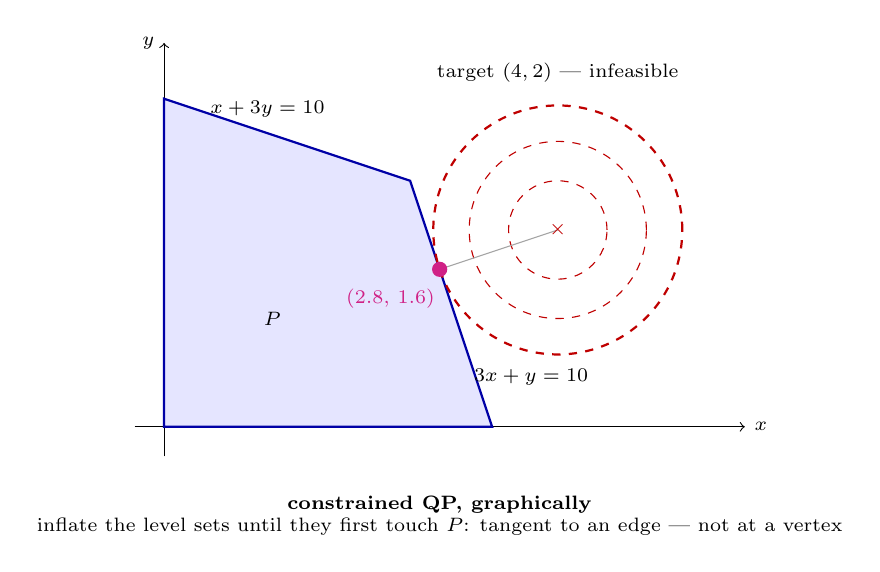
\begin{tikzpicture}[scale=1.25, font=\scriptsize]
  \draw[->] (-0.3,0) -- (5.9,0) node[right] {$x$};
  \draw[->] (0,-0.3) -- (0,3.9) node[left] {$y$};
  \draw[fill=blue!10, draw=blue!65!black, thick] (0,0) -- (3.333,0) -- (2.5,2.5) -- (0,3.333) -- cycle;
  \node at (1.1,1.1) {$P$};
  \node[anchor=west] at (3.05,0.5) {$3x+y=10$};
  \node[anchor=south] at (1.05,3.05) {$x+3y=10$};
  \draw[dashed, red!75!black] (4,2) circle (0.5);
  \draw[dashed, red!75!black] (4,2) circle (0.9);
  \draw[dashed, red!75!black, thick] (4,2) circle (1.2649);
  \draw[gray!70, thin] (4,2) -- (2.8,1.6);
  \node[red!75!black] at (4,2) {$\times$};
  \node[anchor=south] at (4.0,3.4) {target $(4,2)$ --- infeasible};
  \fill[magenta!85!black] (2.8,1.6) circle (2.2pt);
  \node[anchor=north east, magenta!85!black] at (2.85,1.5) {$(2.8,\,1.6)$};
  \node[align=center] at (2.8,-0.9) {\textbf{constrained QP, graphically}\\
    inflate the level sets until they first touch $P$: tangent to an edge --- not at a vertex};
\end{tikzpicture}
\end{center}
\vspace{2pt}

\emph{in the control column of Section 2's table, the same move --- quadratic cost over
linear structure --- is called LQR. same rung, third language.}
\end{board}
\key{\begin{tabular}[t]{@{}l@{}}
1. curved objective $\Rightarrow$ the optimum can leave the vertices: interior (target feasible), edge (here), or vertex. \\
2. it stops wherever the lowest level set first touches $P$ --- LP's flat level sets slide to a corner.
\end{tabular}}
\demo{QP-Graphical-Demo.exe}{two panels: inflate the circle in 2D, watch the bowl in 3D; drag the target --- interior, edge, vertex.}
\demo{week03\_markowitz.ipynb}{week 3's Colab --- Markowitz as a constrained QP; solve it, then trace the frontier.}
{\color{watchink}\small\textbf{read}\quad Caron, \emph{Quadratic Programming in Python} --- same picture, plus solver code.\\
\url{https://scaron.info/blog/quadratic-programming-in-python.html}}
\takeaway{a QP is LP's polyhedron plus a curved bowl: still convex, still local $=$ global --- but the vertex story is over.}

% ---------------------------------------------------------------- 6
\beat{6}{Convexity-preserving operations}
\begin{board}
{\small\emph{(Boyd \& Vandenberghe, }Convex Optimization\emph{, Part I)}}
\vspace{6pt}

$\mathrm{dom}(f) = \{\, x \in \mathbb{R}^n \;:\; f(x) < +\infty \,\}$
\vspace{10pt}

\textbf{Examples of convex functions}
\vspace{5pt}

\begin{tabular}{@{}l@{\qquad}l@{\qquad}l@{}}
\emph{univariate} & affine function      & $ax + b$ \\[4pt]
                  & quadratic function   & $px^{2} + qx + r$ \quad if $p \ge 0$ \\[4pt]
                  & power function       & $x^{\alpha}$ \quad ($\alpha \ge 1$ \ or \ $\alpha \le 0$) \\[4pt]
                  & negative logarithm   & $-\log x$ \\[10pt]
\emph{multivariate} & affine function    & $a^{\top}x + b$ \\[4pt]
                  & quadratic function   & $x^{\top}Px + x^{\top}q + r$ \quad if $P \succeq 0$ \\[4pt]
                  & norm                 & $\|x\|_p$ \quad for $p \ge 1$ \\
\end{tabular}
\vspace{5pt}

\quad $P \succeq 0$ \ (\emph{positive semidefinite}) \ $\iff$ \ $x^{\top}Px \ge 0 \quad \forall x \in \mathbb{R}^n$
\vspace{12pt}

\textbf{Convexity-preserving operations}
\vspace{5pt}

\quad 1) \textbf{Composition with affine functions:}
\vspace{2pt}

\qquad $f(x)$ is convex in $x$, \ then \ $g(x) = f(Ax + b)$ is also convex in $x$.
\vspace{8pt}

\quad 2) \textbf{Nonnegative weighted sum:}
\vspace{2pt}

\qquad $f_1, f_2, \dots, f_k$ are convex in $x$, \ then \ $g(x) = w_1 f_1(x) + \cdots + w_k f_k(x)$
\vspace{1pt}

\qquad is also convex in $x$ \ for \ $w_1, w_2, \dots, w_k \ge 0$.
\vspace{8pt}

\quad 3) \textbf{Pointwise supremum:}
\vspace{2pt}

\qquad If $f(x,y)$ is convex in $x$ for every fixed $y \in Y$,
\vspace{1pt}

\qquad then \ $g(x) = \sup_{y \in Y} f(x,y)$ \ is also convex in $x$.
\vspace{4pt}

\begin{center}
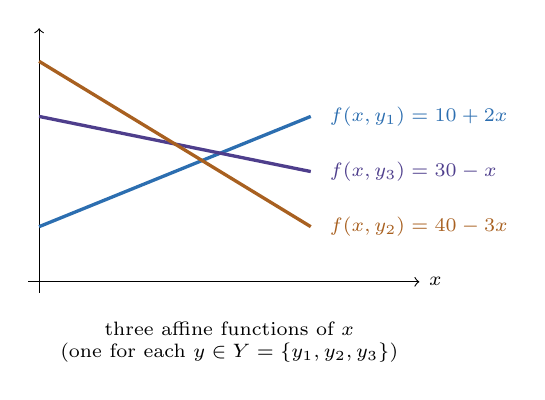
\begin{tikzpicture}[xscale=0.345, yscale=0.070, font=\scriptsize]
  \draw[->] (-0.4,0) -- (14.0,0) node[right] {$x$};
  \draw[->] (0,-2) -- (0,46);
  \draw[lineA, very thick] (0,10) -- (10,30)
       node[right, xshift=3pt, lineA] {$f(x,y_1) = 10 + 2x$};
  \draw[lineC, very thick] (0,30) -- (10,20)
       node[right, xshift=3pt, lineC] {$f(x,y_3) = 30 - x$};
  \draw[lineB, very thick] (0,40) -- (10,10)
       node[right, xshift=3pt, lineB] {$f(x,y_2) = 40 - 3x$};
  \node[align=center] at (7.0,-11) {three affine functions of $x$\\ (one for each $y \in Y = \{y_1,y_2,y_3\}$)};
\end{tikzpicture}
\hspace{6mm}
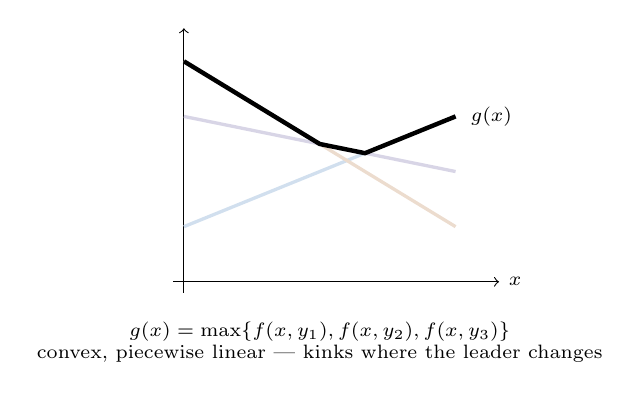
\begin{tikzpicture}[xscale=0.345, yscale=0.070, font=\scriptsize]
  \draw[->] (-0.4,0) -- (11.6,0) node[right] {$x$};
  \draw[->] (0,-2) -- (0,46);
  \draw[lineA!22!white, very thick] (0,10) -- (10,30);
  \draw[lineC!22!white, very thick] (0,30) -- (10,20);
  \draw[lineB!22!white, very thick] (0,40) -- (10,10);
  \draw[black, ultra thick] (0,40) -- (5,25) -- (6.667,23.333) -- (10,30);
  \fill (5,25) circle (2.2pt); \fill (6.667,23.333) circle (2.2pt);
  \node[anchor=west] at (10.2,30) {$g(x)$};
  \node[align=center] at (5.0,-11) {$g(x) = \max\{f(x,y_1), f(x,y_2), f(x,y_3)\}$\\ convex, piecewise linear --- kinks where the leader changes};
\end{tikzpicture}
\end{center}
\vspace{4pt}

\quad 4) \textbf{Partial minimization:}
\vspace{2pt}

\qquad If $f(x,y)$ is \emph{jointly convex} in $x$ and $y$, and $C$ is a convex set,
\vspace{1pt}

\qquad then \ $g(x) = \inf\,\{\, f(x,y) \;:\; y \in C \,\}$ \ is convex in $x$.
\vspace{5pt}

\qquad \emph{jointly convex:} \quad
$f\!\left[\lambda \begin{pmatrix} x_1 \\ y_1 \end{pmatrix}
        + (1-\lambda)\begin{pmatrix} x_2 \\ y_2 \end{pmatrix}\right]
 \;\le\; \lambda f\!\begin{pmatrix} x_1 \\ y_1 \end{pmatrix}
        + (1-\lambda)\, f\!\begin{pmatrix} x_2 \\ y_2 \end{pmatrix}$
\vspace{2pt}

\qquad\qquad $\forall \lambda \in [0,1], \quad \forall \begin{pmatrix} x_1 \\ y_1 \end{pmatrix},
\begin{pmatrix} x_2 \\ y_2 \end{pmatrix}$
\vspace{5pt}

\qquad {\color{punchink}$f(x,y) = xy$ is convex in $x$ and in $y$ separately, but \emph{not} jointly convex.}
\vspace{12pt}

\textbf{Back to what we have already used}
\vspace{5pt}

\begin{tabular}{@{}l@{\qquad}l@{}}
 least squares $\|Ax-b\|_2^2$                  & $\|\cdot\|_2^2$ convex, then (1) \\[5pt]
 piecewise linear $\max_i (a_i^{\top}x + b_i)$ & affine convex, then (3) \\[5pt]
 Markowitz $x^{\top}\Sigma x$                  & quadratic with $\Sigma \succeq 0$ \ ($= \|Lx\|_2^2$ for $\Sigma = L^{\top}L$: (1) again) \\[5pt]
 polyhedron $P = \{x : Ax \le b\}$             & intersection of $m$ half-spaces --- intersection of convex sets is convex \\
\end{tabular}
\end{board}
\takeaway{convexity is compositional: certify the pieces, then check the operation. the risk measures (CVaR, week 4) and worst-case objectives ahead are built exactly this way.}

% ---------------------------------------------------------------- 7
\beat{7}{Probability review}
\begin{board}
back to Section 2's table: the OR column had \textbf{uncertain data} $\xi$. today, the vocabulary ---
textbook notation ($X$, $f$) first, this course's notation ($\tilde\xi$) at the end.
\vspace{10pt}

\textbf{Random variable}
\vspace{4pt}

\bul \textbf{random experiment:} its outcome is not known in advance
\vspace{3pt}

\bul \textbf{sample space} $S$ = the set of all possible outcomes
\vspace{6pt}

\textbf{Def} (\emph{random variable}) \quad a function that assigns a real number to each outcome: \quad $X : S \to \mathbb{R}$
\vspace{3pt}

\quad capital $X$ = the random variable, \qquad lowercase $x$ = a value it takes
\vspace{5pt}

\quad toss a coin twice: \ $S = \{HH, HT, TH, TT\}$, \ each outcome has probability $\tfrac14$
\vspace{3pt}

\quad $X$ = number of heads: \quad $X(HH) = 2, \quad X(HT) = 1, \quad X(TH) = 1, \quad X(TT) = 0$
\vspace{6pt}

\begin{center}
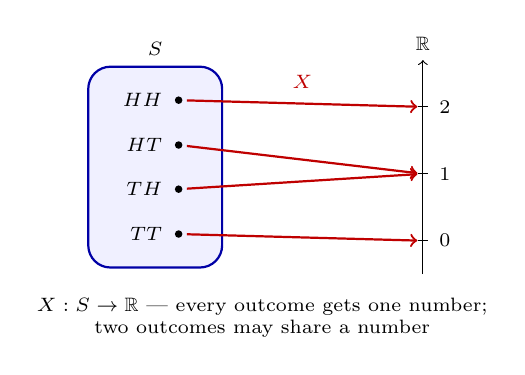
\begin{tikzpicture}[scale=0.85, font=\scriptsize]
  \draw[rounded corners=8pt, fill=blue!6, draw=blue!65!black, thick] (0,0) rectangle (2.0,3.0);
  \node[anchor=south] at (1.0,3.02) {$S$};
  \foreach \y/\lab in {2.5/HH, 1.83/HT, 1.17/TH, 0.5/TT}
    { \fill (1.35,\y) circle (1.6pt); \node[anchor=east] at (1.25,\y) {$\lab$}; }
  \draw[->] (5.0,-0.1) -- (5.0,3.1) node[above] {$\mathbb{R}$};
  \foreach \v/\y in {0/0.4, 1/1.4, 2/2.4}
    { \draw (4.92,\y) -- (5.08,\y); \node[anchor=west] at (5.1,\y) {$\v$}; }
  \draw[->, red!75!black, thick, shorten >=2pt, shorten <=3pt] (1.35,2.5)  -- (5.0,2.4);
  \draw[->, red!75!black, thick, shorten >=2pt, shorten <=3pt] (1.35,1.83) -- (5.0,1.4);
  \draw[->, red!75!black, thick, shorten >=2pt, shorten <=3pt] (1.35,1.17) -- (5.0,1.4);
  \draw[->, red!75!black, thick, shorten >=2pt, shorten <=3pt] (1.35,0.5)  -- (5.0,0.4);
  \node[red!75!black] at (3.2,2.78) {$X$};
  \node[align=center] at (2.6,-0.75) {$X : S \to \mathbb{R}$ --- every outcome gets one number;\\ two outcomes may share a number};
\end{tikzpicture}
\hspace{12mm}
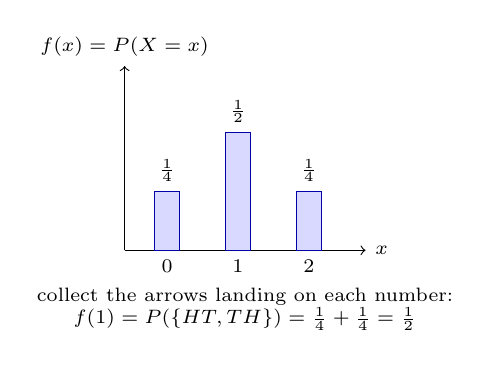
\begin{tikzpicture}[xscale=0.9, yscale=3.0, font=\scriptsize]
  \draw[->] (-0.6,0) -- (2.8,0) node[right] {$x$};
  \draw[->] (-0.6,0) -- (-0.6,0.78) node[above] {$f(x) = P(X = x)$};
  \draw[fill=blue!15, draw=blue!65!black] (-0.18,0) rectangle (0.18,0.25);
  \draw[fill=blue!15, draw=blue!65!black] (0.82,0) rectangle (1.18,0.5);
  \draw[fill=blue!15, draw=blue!65!black] (1.82,0) rectangle (2.18,0.25);
  \node[below] at (0,0) {$0$}; \node[below] at (1,0) {$1$}; \node[below] at (2,0) {$2$};
  \node[above, font=\tiny] at (0,0.25) {$\tfrac14$};
  \node[above, font=\tiny] at (1,0.5) {$\tfrac12$};
  \node[above, font=\tiny] at (2,0.25) {$\tfrac14$};
  \node[align=center] at (1.1,-0.25) {collect the arrows landing on each number:\\ $f(1) = P(\{HT, TH\}) = \tfrac14 + \tfrac14 = \tfrac12$};
\end{tikzpicture}
\end{center}
\vspace{6pt}

\bul \textbf{discrete} $X$: countably many values --- number of defective parts, number of arrivals, demand
\vspace{3pt}

\bul \textbf{continuous} $X$: values fill an interval --- length, time, temperature, a return
\vspace{14pt}

\textbf{Discrete random variables}
\vspace{5pt}

\textbf{Def} (\emph{probability mass function, PMF}) \quad
$f(x) = P(X = x)$, \qquad $f : \mathbb{R} \to [0,1]$
\vspace{3pt}

\quad (1) \ $f(x) \ge 0$ \qquad (2) \ $\sum_x f(x) = 1$ \qquad\qquad $P(X \in A) = \sum_{x \in A} f(x)$
\vspace{3pt}

\quad two coins: \ $f(0) = \tfrac14$, \ $f(1) = \tfrac12$, \ $f(2) = \tfrac14$, \qquad
$P(X \ge 1) = f(1) + f(2) = \tfrac34$
\vspace{8pt}

\textbf{Def} (\emph{mean, variance})
\vspace{3pt}

\quad mean: \quad $\mu = \mathbb{E}[X] = \sum_x x\, f(x)$
\vspace{3pt}

\quad variance: \quad $\sigma^2 = \mathrm{Var}(X) = \sum_x (x - \mu)^2 f(x) = \mathbb{E}[X^2] - \mu^2$,
\qquad standard deviation \ $\sigma = \sqrt{\mathrm{Var}(X)}$
\vspace{3pt}

\quad function of $X$: \quad $\mathbb{E}[h(X)] = \sum_x h(x)\, f(x)$
\qquad {\color{punchink}\small $\leftarrow$ law of the unconscious statistician}
\vspace{3pt}

\quad $\mathbb{E}[aX + b] = a\,\mathbb{E}[X] + b$, \qquad $\mathrm{Var}(aX + b) = a^2\,\mathrm{Var}(X)$
\vspace{10pt}

\textbf{Example 1} \quad demand $X$ for a spare part next month:
\vspace{5pt}

\begin{center}
\begin{tabular}{@{}l|ccc@{}}
 $x$     & 4    & 8   & 12   \\ \hline
 $f(x)$  & 0.25 & 0.5 & 0.25 \\
\end{tabular}
\qquad\qquad
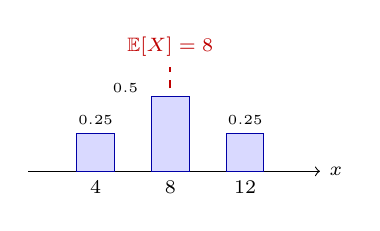
\begin{tikzpicture}[scale=0.95, font=\scriptsize, baseline=-6pt]
  \draw[dashed, red!75!black, thick] (1.6,0) -- (1.6,1.4) node[above] {$\mathbb{E}[X] = 8$};
  \draw[->] (-0.3,0) -- (3.6,0) node[right] {$x$};
  \draw[fill=blue!15, draw=blue!65!black] (0.35,0) rectangle (0.85,0.5);
  \draw[fill=blue!15, draw=blue!65!black] (1.35,0) rectangle (1.85,1.0);
  \draw[fill=blue!15, draw=blue!65!black] (2.35,0) rectangle (2.85,0.5);
  \node[below] at (0.6,0) {4}; \node[below] at (1.6,0) {8}; \node[below] at (2.6,0) {12};
  \node[font=\tiny] at (0.6,0.68) {$0.25$}; \node[font=\tiny, anchor=east] at (1.30,1.12) {$0.5$}; \node[font=\tiny] at (2.6,0.68) {$0.25$};
\end{tikzpicture}
\end{center}
\vspace{5pt}

\quad $\mathbb{E}[X] = 0.25 \cdot 4 + 0.5 \cdot 8 + 0.25 \cdot 12 = 8$
\vspace{3pt}

\quad $\mathrm{Var}(X) = 0.25 \cdot (4 - 8)^2 + 0.5 \cdot (8 - 8)^2 + 0.25 \cdot (12 - 8)^2 = 8$,
\qquad $\sigma = 2\sqrt{2} \approx 2.83$
\vspace{14pt}

\textbf{Continuous random variables}
\vspace{5pt}

\textbf{Def} (\emph{probability density function, PDF}) \quad $f : \mathbb{R} \to \mathbb{R}_+$ with
\vspace{3pt}

\quad (1) \ $f(x) \ge 0$ \qquad (2) \ $\int_{-\infty}^{\infty} f(x)\, dx = 1$ \qquad
(3) \ $P(a \le X \le b) = \int_a^b f(x)\, dx$ \ = area under $f$ from $a$ to $b$
\vspace{3pt}

\quad {\color{punchink}$f(x)$ is \emph{not} a probability:} \ $P(X = x) = 0$ for every single $x$, \ and $f(x) > 1$ is allowed
\vspace{8pt}

\textbf{Def} (\emph{mean, variance}) \quad same as discrete --- the sums become integrals:
\vspace{3pt}

\quad $\mu = \mathbb{E}[X] = \int x\, f(x)\, dx$, \qquad
$\sigma^2 = \mathrm{Var}(X) = \int (x - \mu)^2 f(x)\, dx = \mathbb{E}[X^2] - \mu^2$, \qquad
$\mathbb{E}[h(X)] = \int h(x)\, f(x)\, dx$
\vspace{10pt}

\textbf{Example 2} \quad $X \sim \mathrm{Uniform}[a,b]$ \ ---
$f(x) = \dfrac{1}{b-a}$ \ on \ $[a,b]$, \ $0$ outside
\vspace{4pt}

\begin{center}
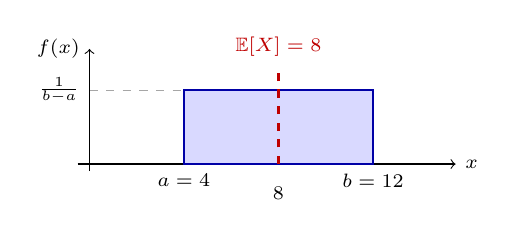
\begin{tikzpicture}[xscale=0.30, yscale=7.5, font=\scriptsize]
  \draw[dashed, gray!70] (0,0.125) -- (4,0.125);
  \draw[->] (-0.5,0) -- (15.5,0) node[right] {$x$};
  \draw[->] (0,-0.012) -- (0,0.195) node[left] {$f(x)$};
  \draw[fill=blue!15, draw=blue!65!black, thick] (4,0) rectangle (12,0.125);
  \node[below] at (4,0) {$a = 4$};
  \node[below] at (12,0) {$b = 12$};
  \node[left] at (0,0.125) {$\tfrac{1}{b-a}$};
  \draw[dashed, red!75!black, thick] (8,0) -- (8,0.165) node[above] {$\mathbb{E}[X] = 8$};
  \node[below] at (8,-0.022) {$8$};
\end{tikzpicture}
\end{center}
\vspace{4pt}

\quad mean:
\[
\mathbb{E}[X] \;=\; \int_a^b x \, \frac{1}{b-a} \, dx
 \;=\; \frac{1}{b-a}\left[\frac{x^2}{2}\right]_a^b
 \;=\; \frac{b^2 - a^2}{2(b-a)} \;=\; \frac{a+b}{2}
\]

\quad second moment --- $h(x) = x^2$:
\[
\mathbb{E}[X^2] \;=\; \int_a^b x^2 \, \frac{1}{b-a} \, dx
 \;=\; \frac{1}{b-a}\left[\frac{x^3}{3}\right]_a^b
 \;=\; \frac{b^3 - a^3}{3(b-a)} \;=\; \frac{a^2 + ab + b^2}{3}
\]

\quad variance --- subtract, no new integral:
\[
\mathrm{Var}(X) \;=\; \mathbb{E}[X^2] - \mathbb{E}[X]^2
 \;=\; \frac{a^2 + ab + b^2}{3} - \frac{(a+b)^2}{4}
 \;=\; \frac{(b-a)^2}{12}
\]

\quad with $a = 4$, $b = 12$: \qquad
$\mathbb{E}[X] = 8$, \qquad
$\mathrm{Var}(X) = \dfrac{64}{12} = \dfrac{16}{3}$, \qquad
$\sigma = \dfrac{4}{\sqrt{3}} \approx 2.31$
\vspace{12pt}

\textbf{Normal distribution} \quad $X \sim \mathcal{N}(\mu, \sigma^2)$:
\qquad $f(x) = \dfrac{1}{\sigma\sqrt{2\pi}}\, \exp\!\Big(\!-\dfrac{(x-\mu)^2}{2\sigma^2}\Big)$, \ $x \in \mathbb{R}$
\vspace{4pt}

\quad $\mathbb{E}[X] = \mu$, \qquad $\mathrm{Var}(X) = \sigma^2$
\vspace{3pt}

\quad $P(\mu - \sigma \le X \le \mu + \sigma) \approx 0.68$, \qquad
$P(\mu - 2\sigma \le X \le \mu + 2\sigma) \approx 0.95$
\vspace{4pt}

\begin{center}
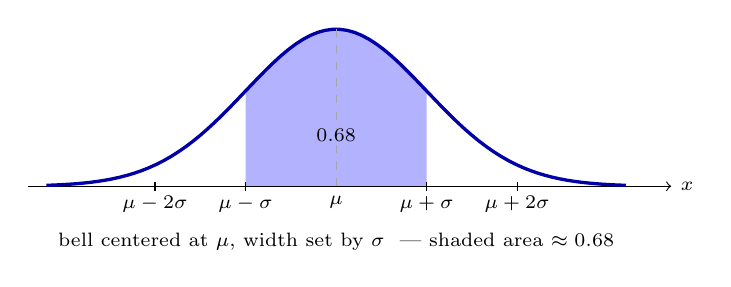
\begin{tikzpicture}[xscale=1.15, yscale=5.0, font=\scriptsize]
  \fill[blue!30, domain=-1:1, samples=40] (-1,0) -- plot (\x, {0.3989*exp(-\x*\x/2)}) -- (1,0) -- cycle;
  \draw[->] (-3.4,0) -- (3.7,0) node[right] {$x$};
  \draw[very thick, blue!65!black, domain=-3.2:3.2, samples=80] plot (\x, {0.3989*exp(-\x*\x/2)});
  \draw[dashed, gray!70] (0,0) -- (0,0.3989);
  \foreach \t in {-2,-1,1,2} \draw (\t,0.012) -- (\t,-0.012);
  \node[below] at (0,0) {$\mu$};
  \node[below] at (-1,0) {$\mu - \sigma$}; \node[below] at (1,0) {$\mu + \sigma$};
  \node[below] at (-2,0) {$\mu - 2\sigma$}; \node[below] at (2,0) {$\mu + 2\sigma$};
  \node at (0,0.13) {$0.68$};
  \node at (0,-0.14) {bell centered at $\mu$, width set by $\sigma$ \ --- shaded area $\approx 0.68$};
\end{tikzpicture}
\end{center}
\vspace{14pt}

\textbf{Two random variables}
\vspace{5pt}

\textbf{Def} (\emph{joint PMF}) \quad
$f_{XY}(x, y) = P(X = x, \ Y = y)$, \qquad $f_{XY} \ge 0$, \qquad $\sum_x \sum_y f_{XY}(x, y) = 1$
\vspace{6pt}

\textbf{Def} (\emph{marginal PMF}) \quad
$f_X(x) = \sum_y f_{XY}(x, y)$, \qquad $f_Y(y) = \sum_x f_{XY}(x, y)$
\vspace{2pt}

\quad --- row sums and column sums, written in the \emph{margins} of the table
\vspace{10pt}

\textbf{Example 3} \quad two assets, returns tomorrow: \ $X$, $Y$ each either down ($-0.10$) or up ($+0.20$)
\vspace{6pt}

\begin{center}
\begin{tabular}{@{}c|cc|c@{}}
 $f_{XY}(x, y)$        & $y = -0.10$ & $y = 0.20$ & $f_X(x)$ \\ \hline
 $x = -0.10$           & $0.3$ & $0.2$ & $0.5$ \\
 $x = \phantom{-}0.20$ & $0.2$ & $0.3$ & $0.5$ \\ \hline
 $f_Y(y)$              & $0.5$ & $0.5$ & $1$ \\
\end{tabular}
\end{center}
\vspace{4pt}

\quad each asset alone: down or up w.p.\ $\tfrac12$. \quad together: same direction w.p.\ $0.3 + 0.3 = 0.6$
\vspace{10pt}

\textbf{Def} (\emph{joint PDF}) \quad
$f_{XY} : \mathbb{R}^2 \to \mathbb{R}_+$, \qquad $\iint f_{XY}(x, y)\, dx\, dy = 1$, \qquad
$P\big((X, Y) \in R\big) = \iint_R f_{XY}(x, y)\, dx\, dy$
\vspace{2pt}

\quad --- the \textbf{volume} under $f_{XY}$ above the region $R$
\vspace{3pt}

\quad marginal PDF: \ $f_X(x) = \int f_{XY}(x, y)\, dy$ \quad --- the sum becomes an integral
\vspace{10pt}

\textbf{Example 4} \quad $(X, Y)$ uniform on the unit square: \quad $f_{XY}(x, y) = 1$ \ on $[0,1]^2$, \ $0$ outside
\vspace{4pt}

\begin{center}
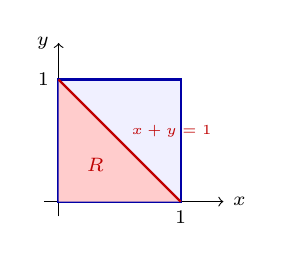
\begin{tikzpicture}[scale=1.55, font=\scriptsize, baseline=(b)]
  \coordinate (b) at (0,0.5);
  \draw[->] (-0.12,0) -- (1.35,0) node[right] {$x$};
  \draw[->] (0,-0.12) -- (0,1.3) node[left] {$y$};
  \draw[fill=blue!6, draw=blue!65!black, thick] (0,0) rectangle (1,1);
  \fill[red!20] (0,0) -- (1,0) -- (0,1) -- cycle;
  \draw[red!75!black, thick] (1,0) -- (0,1);
  \node[red!75!black] at (0.3,0.3) {$R$};
  \node[below] at (1,0) {$1$}; \node[left] at (0,1) {$1$};
  \node[anchor=west, font=\tiny, red!75!black] at (0.52,0.58) {$x + y = 1$};
\end{tikzpicture}
\qquad\quad
\begin{minipage}{0.62\textwidth}
$P(X + Y \le 1) = \iint_R 1 \; dx\, dy$ = area of the triangle $R$ $= \tfrac12$
\vspace{6pt}

marginal: \ $f_X(x) = \int_0^1 1 \; dy = 1$ on $[0,1]$ --- $X$ alone is Uniform$[0,1]$
\end{minipage}
\end{center}
\vspace{10pt}

\textbf{Def} (\emph{independence}) \quad $X$, $Y$ are independent if \quad
$f_{XY}(x, y) = f_X(x)\, f_Y(y) \quad \forall\, x, y$ \qquad (PMF or PDF)
\vspace{3pt}

\quad Example 3: \ $f_{XY}(-0.10, -0.10) = 0.3 \ne 0.5 \cdot 0.5$ \ --- \textbf{not} independent
\vspace{2pt}

\quad Example 4: \ $f_{XY}(x, y) = 1 = 1 \cdot 1$ \ --- independent
\vspace{10pt}

\textbf{Def} (\emph{covariance, correlation})
\vspace{3pt}

\quad $\mathrm{Cov}(X, Y) = \mathbb{E}\big[(X - \mu_X)(Y - \mu_Y)\big] = \mathbb{E}[XY] - \mu_X \mu_Y$,
\qquad $\mathrm{Cov}(X, X) = \mathrm{Var}(X)$
\vspace{3pt}

\quad $\rho_{XY} = \dfrac{\mathrm{Cov}(X, Y)}{\sigma_X\, \sigma_Y}$, \qquad $-1 \le \rho_{XY} \le 1$
\vspace{3pt}

\quad $\rho > 0$: move together, \quad $\rho < 0$: move opposite, \quad independent $\Rightarrow$ $\rho = 0$
\vspace{4pt}

\begin{center}
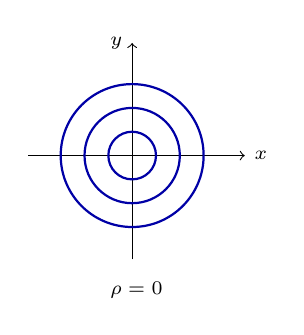
\begin{tikzpicture}[scale=0.55, font=\scriptsize]
  \draw[->] (-2.4,0) -- (2.6,0) node[right] {$x$};
  \draw[->] (0,-2.4) -- (0,2.6) node[left] {$y$};
  \foreach \c in {0.55,1.1,1.65}
    \draw[blue!65!black, thick] (0,0) circle (\c);
  \node at (0.1,-3.1) {$\rho = 0$};
\end{tikzpicture}
\hspace{9mm}
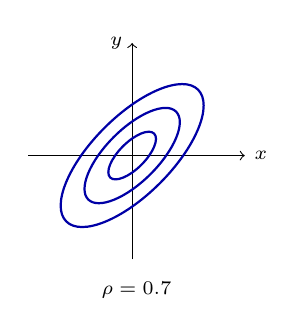
\begin{tikzpicture}[scale=0.55, font=\scriptsize]
  \draw[->] (-2.4,0) -- (2.6,0) node[right] {$x$};
  \draw[->] (0,-2.4) -- (0,2.6) node[left] {$y$};
  \foreach \c in {0.55,1.1,1.65}
    \draw[blue!65!black, thick, rotate=45] (0,0) ellipse ({1.304*\c} and {0.548*\c});
  \node at (0.1,-3.1) {$\rho = 0.7$};
\end{tikzpicture}
\hspace{9mm}
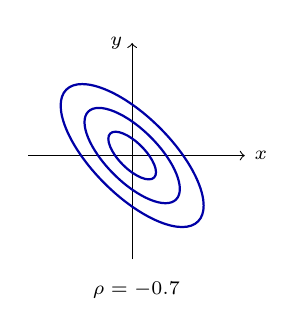
\begin{tikzpicture}[scale=0.55, font=\scriptsize]
  \draw[->] (-2.4,0) -- (2.6,0) node[right] {$x$};
  \draw[->] (0,-2.4) -- (0,2.6) node[left] {$y$};
  \foreach \c in {0.55,1.1,1.65}
    \draw[blue!65!black, thick, rotate=-45] (0,0) ellipse ({1.304*\c} and {0.548*\c});
  \node at (0.1,-3.1) {$\rho = -0.7$};
\end{tikzpicture}\\[2pt]
{\scriptsize contours of the joint PDF of two normal random variables, \ $\mu_X = \mu_Y = 0$, \ $\sigma_X = \sigma_Y = 1$}
\end{center}
\vspace{8pt}

\textbf{Example 3, continued} \quad (use the margins for $\mu$ and $\sigma$, all four cells for the covariance)
\vspace{4pt}

\quad $\mu_X = 0.5 \cdot (-0.10) + 0.5 \cdot 0.20 = 0.05$, \qquad $\mu_Y = 0.05$
\vspace{3pt}

\quad $\mathrm{Var}(X) = 0.5 \cdot (-0.15)^2 + 0.5 \cdot (0.15)^2 = 0.0225$, \qquad $\sigma_X = \sigma_Y = 0.15$
\[
\begin{aligned}
\mathrm{Cov}(X, Y)
 &= 0.3\,(-0.15)(-0.15) + 0.2\,(-0.15)(0.15) + 0.2\,(0.15)(-0.15) + 0.3\,(0.15)(0.15) \\
 &= (0.3 - 0.2 - 0.2 + 0.3) \cdot 0.0225 \;=\; 0.0045
\end{aligned}
\]

\quad $\rho_{XY} = \dfrac{0.0045}{0.15 \cdot 0.15} = 0.2$ \quad --- the two assets tend to move together
\vspace{14pt}

\textbf{Linear combinations}
\vspace{4pt}

\quad $\mathbb{E}[aX + bY] = a\,\mu_X + b\,\mu_Y$ \qquad --- always, no independence needed
\vspace{3pt}

\quad $\mathrm{Var}(aX + bY) = a^2\,\mathrm{Var}(X) + b^2\,\mathrm{Var}(Y) + 2ab\,\mathrm{Cov}(X, Y)$
\vspace{8pt}

\quad $n$ random variables $X = (X_1, \dots, X_n)$:
\vspace{3pt}

\qquad mean vector \ $\mu = \big(\mathbb{E}[X_1], \dots, \mathbb{E}[X_n]\big)^{\top} \in \mathbb{R}^n$
\vspace{3pt}

\qquad covariance matrix \ $\Sigma \in \mathbb{R}^{n \times n}$, \ $\Sigma_{ij} = \mathrm{Cov}(X_i, X_j)$;
\ diagonal $\Sigma_{ii} = \mathrm{Var}(X_i)$; \ symmetric; \ always $\Sigma \succeq 0$
\vspace{4pt}

\quad for fixed $c \in \mathbb{R}^n$: \qquad
$\mathbb{E}[c^{\top}X] = c^{\top}\mu$, \qquad $\mathrm{Var}(c^{\top}X) = c^{\top}\Sigma c$
\vspace{4pt}

\quad $n = 2$, \ $c = (a, b)$: \quad
$c^{\top}\Sigma c
 = \begin{pmatrix} a & b \end{pmatrix}
   \begin{pmatrix} \mathrm{Var}(X) & \mathrm{Cov}(X,Y) \\ \mathrm{Cov}(X,Y) & \mathrm{Var}(Y) \end{pmatrix}
   \begin{pmatrix} a \\ b \end{pmatrix}$
\ --- $\mathrm{Var}(aX + bY)$ again
\vspace{4pt}

\quad Example 3: \quad
$\mu = \begin{pmatrix} 0.05 \\ 0.05 \end{pmatrix}$, \qquad
$\Sigma = \begin{pmatrix} 0.0225 & 0.0045 \\ 0.0045 & 0.0225 \end{pmatrix}$
\vspace{14pt}

\textbf{In this course's notation} \quad the decision is already $x$, so the uncertain data gets its own letter:
\vspace{5pt}

\begin{center}
\renewcommand{\arraystretch}{1.25}
\begin{tabular}{@{}l|l|l@{}}
                        & textbook                      & this course \\ \hline
random variable         & $X$                           & $\tilde\xi$, \ with distribution $\mathbb{P}$: \ $\tilde\xi \sim \mathbb{P}$ \\
a value of it           & $x$                           & $\xi$ \ (a \emph{realization}) \\
probability             & $P(\cdot)$                    & $\mathbb{P}(\cdot)$ \\
set of possible values  & range of $X$                  & support $\Xi$ \ (smallest closed set with $\mathbb{P}(\tilde\xi \in \Xi) = 1$) \\
discrete                & values $x$, PMF $f(x)$        & scenarios $\xi_1, \dots, \xi_S$ with probabilities $p_1, \dots, p_S$ \\
continuous              & PDF $f(x)$                    & density $p(\xi)$ \\
mean, discrete          & $\sum_x x\, f(x)$             & $\mathbb{E}[\tilde\xi] = \sum_{s \in [S]} p_s\, \xi_s$ \\
mean, continuous        & $\int x\, f(x)\, dx$          & $\mathbb{E}[\tilde\xi] = \int_{\Xi} \xi\, p(\xi)\, d\xi$ \\
function of it          & $\mathbb{E}[h(X)]$            & $\mathbb{E}[f(\tilde\xi)]$ \ ($f$ = any function, e.g.\ a cost --- not a PDF) \\
random vector           & $X \in \mathbb{R}^k$, \ $\mu$, $\Sigma$ & $\tilde\xi \in \mathbb{R}^k$, \ $\mu$, $\Sigma$ \\
\end{tabular}
\end{center}
\vspace{12pt}

\textbf{The bridge to optimization} \quad data random $\Rightarrow$ cost random:
$f(x, \tilde\xi)$ is a random variable, \ $\mathbb{E}[f(x,\tilde\xi)]$ is a number.
\[
\min_x \;\; \mathbb{E}\big[f(x, \tilde\xi)\big]
\]
\end{board}
\takeaway{every paradigm in this course differs in one place only: \emph{how} it collapses the randomness to a number.}

% ---------------------------------------------------------------- 8
\beat{8}{Running example: the Markowitz portfolio}
\begin{board}
a budget of $1$, \ $n$ assets. \quad decide the split today; the returns are revealed tomorrow.
\vspace{6pt}

\bul \textbf{decision:} \ $x \in \mathbb{R}^n$, \ $x_j$ = share of the budget in asset $j$
\vspace{3pt}

\bul \textbf{uncertain data:} \ $\tilde\xi = (\tilde\xi_1, \dots, \tilde\xi_n) \in \mathbb{R}^n$, \
      $\tilde\xi_j$ = return of asset $j$ \ --- a random vector with mean $\mu$, covariance matrix $\Sigma$
\vspace{3pt}

\bul \textbf{feasible set:} \ $X = \{\, x \in \mathbb{R}^n \;:\; \mathbf{1}^{\top}x = 1, \ x \ge 0 \,\}$
      \qquad ($\mathbf{1}$ = all-ones vector, \ $\mathbf{1}^{\top}x = x_1 + \cdots + x_n$)
\vspace{10pt}

\textbf{Portfolio return} \quad
$\tilde\xi^{\top}x = x_1\tilde\xi_1 + \cdots + x_n\tilde\xi_n$ \quad --- a random variable
\vspace{3pt}

\quad as a function: \ fix $x$, \quad $f(\xi) = \xi^{\top}x$, \quad $f : \mathbb{R}^n \to \mathbb{R}$
\quad --- Section 0's inner product, fed a random input
\vspace{3pt}

\quad loss: \ $f(x, \tilde\xi) = -\tilde\xi^{\top}x$ \qquad (a gain is a negative loss)
\vspace{6pt}

\quad Section 7's linear combinations with $c = x$: \qquad
$\mathbb{E}[\tilde\xi^{\top}x] = \mu^{\top}x$, \qquad $\mathrm{Var}(\tilde\xi^{\top}x) = x^{\top}\Sigma x$
\vspace{10pt}

\textbf{Check on Example 3} \quad $(\tilde\xi_1, \tilde\xi_2)$ = Example 3's $(X, Y)$, \ half in each: \ $x = (\tfrac12, \tfrac12)$
\vspace{4pt}

\begin{center}
\begin{tabular}{@{}cc|c|c@{}}
 $\xi_1$ & $\xi_2$ & $\tfrac12\xi_1 + \tfrac12\xi_2$ & probability \\ \hline
 $-0.10$ & $-0.10$ & $-0.10$ & $0.3$ \\
 $-0.10$ & $\phantom{-}0.20$ & $\phantom{-}0.05$ & $0.2$ \\
 $\phantom{-}0.20$ & $-0.10$ & $\phantom{-}0.05$ & $0.2$ \\
 $\phantom{-}0.20$ & $\phantom{-}0.20$ & $\phantom{-}0.20$ & $0.3$ \\
\end{tabular}
\qquad\quad $\Rightarrow$ \quad PMF of $\tilde\xi^{\top}x$: \quad
\begin{tabular}{@{}l|ccc@{}}
 value       & $-0.10$ & $0.05$ & $0.20$ \\ \hline
 probability & $0.3$   & $0.4$  & $0.3$  \\
\end{tabular}
\end{center}
\vspace{4pt}

\[
\begin{aligned}
\text{from the PMF:}\quad
 & \mathbb{E}[\tilde\xi^{\top}x] = 0.3\,(-0.10) + 0.4\,(0.05) + 0.3\,(0.20) = 0.05 \\
 & \mathrm{Var}(\tilde\xi^{\top}x) = 0.3\,(-0.15)^2 + 0.4\,(0)^2 + 0.3\,(0.15)^2 = 0.0135 \\[5pt]
\text{from $\mu$ and $\Sigma$:}\quad
 & \mu^{\top}x = \tfrac12\,(0.05) + \tfrac12\,(0.05) = 0.05 \ \checkmark \\
 & x^{\top}\Sigma x = \tfrac14\,(0.0225) + \tfrac14\,(0.0225) + 2 \cdot \tfrac14\,(0.0045) = 0.0135 \ \checkmark
\end{aligned}
\]
\vspace{2pt}

\begin{center}
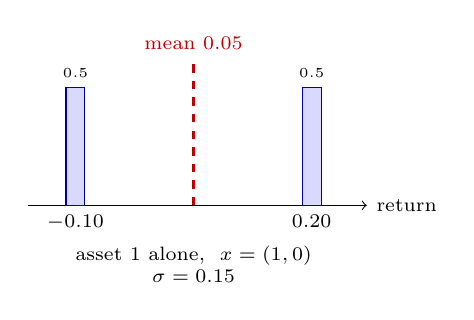
\begin{tikzpicture}[scale=1.0, font=\scriptsize]
  % x-coordinate = 10 x return, y-coordinate = 3 x probability
  \draw[->] (-1.6,0) -- (2.7,0) node[right] {return};
  \draw[fill=blue!15, draw=blue!65!black] (-1.12,0) rectangle (-0.88,1.5);
  \draw[fill=blue!15, draw=blue!65!black] (1.88,0) rectangle (2.12,1.5);
  \draw[dashed, red!75!black, thick] (0.5,0) -- (0.5,1.85) node[above] {mean $0.05$};
  \node[below] at (-1,0) {$-0.10$}; \node[below] at (2,0) {$0.20$};
  \node[above, font=\tiny] at (-1,1.5) {$0.5$}; \node[above, font=\tiny] at (2,1.5) {$0.5$};
  \node[align=center] at (0.5,-0.75) {asset 1 alone, \ $x = (1, 0)$\\ $\sigma = 0.15$};
\end{tikzpicture}
\hspace{16mm}
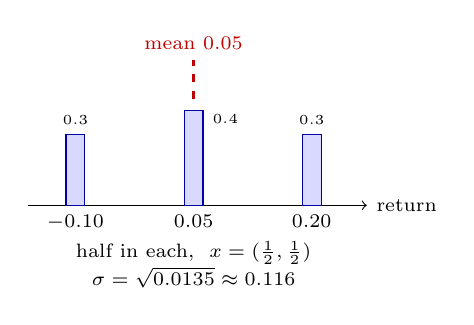
\begin{tikzpicture}[scale=1.0, font=\scriptsize]
  \draw[->] (-1.6,0) -- (2.7,0) node[right] {return};
  \draw[fill=blue!15, draw=blue!65!black] (-1.12,0) rectangle (-0.88,0.9);
  \draw[fill=blue!15, draw=blue!65!black] (0.38,0) rectangle (0.62,1.2);
  \draw[fill=blue!15, draw=blue!65!black] (1.88,0) rectangle (2.12,0.9);
  \draw[dashed, red!75!black, thick] (0.5,1.35) -- (0.5,1.85) node[above] {mean $0.05$};
  \node[below] at (-1,0) {$-0.10$}; \node[below] at (0.5,0) {$0.05$}; \node[below] at (2,0) {$0.20$};
  \node[above, font=\tiny] at (-1,0.9) {$0.3$}; \node[right, font=\tiny] at (0.62,1.1) {$0.4$};
  \node[above, font=\tiny] at (2,0.9) {$0.3$};
  \node[align=center] at (0.5,-0.75) {half in each, \ $x = (\tfrac12, \tfrac12)$\\ $\sigma = \sqrt{0.0135} \approx 0.116$};
\end{tikzpicture}
\end{center}
\vspace{4pt}

\quad same mean, less spread: \textbf{diversification}. \ it comes from $\rho < 1$ --- with $\rho = 1$, \ $x^{\top}\Sigma x$ would stay $0.0225$.
\vspace{12pt}

\textbf{The model} \quad (Markowitz, 1952) \quad --- least risk, subject to an expected-return target $r$:
\[
\begin{aligned}
  \min_x\quad & x^{\top}\Sigma x && \text{variance of the return (risk)}\\
  \text{s.t.}\quad & \mu^{\top}x \ge r && \text{expected return meets the target}\\
                   & \mathbf{1}^{\top}x = 1, \quad x \ge 0 && x \in X
\end{aligned}
\]

\quad Section 5's QP with $Q = 2\Sigma$, $c = 0$; \ convex because $\Sigma \succeq 0$ (Section 6).
\vspace{3pt}

\quad in the language of the bridge: the loss $-\tilde\xi^{\top}x$ is random; Markowitz collapses it with two numbers ---
\vspace{1pt}

\qquad its variance (objective) and its mean (constraint).
\vspace{12pt}

\textbf{Data --- the coding session} \quad $n = 3$, \ $r = 0.10$
\vspace{5pt}

\begin{center}
\begin{tabular}{@{}l|c|c|c@{}}
 asset $j$ & expected return $\mu_j$ & variance $\Sigma_{jj}$ & $\sigma_j = \sqrt{\Sigma_{jj}}$ \\ \hline
 bond      & $0.06$ & $0.010$ & $0.10$ \\
 tech      & $0.10$ & $0.040$ & $0.20$ \\
 energy    & $0.15$ & $0.090$ & $0.30$ \\
\end{tabular}
\end{center}
\vspace{4pt}

\[
x = \begin{pmatrix} x_{\text{bond}} \\ x_{\text{tech}} \\ x_{\text{energy}} \end{pmatrix},
\qquad
\mu = \begin{pmatrix} 0.06 \\ 0.10 \\ 0.15 \end{pmatrix},
\qquad
\Sigma = \begin{pmatrix} 0.010 & 0.001 & 0 \\ 0.001 & 0.040 & 0.015 \\ 0 & 0.015 & 0.090 \end{pmatrix}
\]

\quad covariances: \ bond--tech $0.001$, \ tech--energy $0.015$, \ bond--energy $0$
\vspace{6pt}

\quad written out term by term --- exactly the lines typed in the code:
\[
\begin{aligned}
  \min\quad & 0.010\,x_{\text{bond}}^2 + 0.040\,x_{\text{tech}}^2 + 0.090\,x_{\text{energy}}^2
              + 2(0.001)\,x_{\text{bond}}x_{\text{tech}} + 2(0.015)\,x_{\text{tech}}x_{\text{energy}} \\
  \text{s.t.}\quad & 0.06\,x_{\text{bond}} + 0.10\,x_{\text{tech}} + 0.15\,x_{\text{energy}} \ge 0.10 \\
                   & x_{\text{bond}} + x_{\text{tech}} + x_{\text{energy}} \le 1 \\
                   & x_{\text{bond}},\ x_{\text{tech}},\ x_{\text{energy}} \ge 0
\end{aligned}
\]

\quad budget ``$\le 1$'': leftover sits in cash earning $0$ --- never helps, so the sum is $1$ at the optimum
\vspace{6pt}

\textbf{Solution}
\vspace{3pt}

\quad $\boxed{x^{\star} \approx (0.39,\ 0.29,\ 0.31), \qquad x^{\star\top}\Sigma x^{\star} \approx 0.0169, \qquad \sigma \approx 0.130}$
\qquad $\mu^{\top}x^{\star} = 0.10$ --- target met exactly
\vspace{4pt}

\quad all in tech: \ same expected return $0.10$, \ but $\sigma = 0.20$. \quad the mix cuts $\sigma$ by about a third.
\vspace{3pt}

\quad every asset gets a share --- not a vertex (Section 5).
\vspace{6pt}

\begin{center}
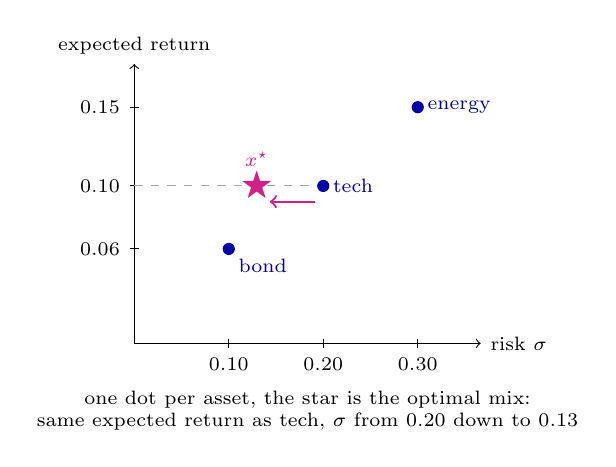
\begin{tikzpicture}[scale=1.0, font=\scriptsize]
  % x-coordinate = 12 x sigma, y-coordinate = 20 x mean
  \draw[->] (0,0) -- (4.4,0) node[right] {risk $\sigma$};
  \draw[->] (0,0) -- (0,3.55) node[above] {expected return};
  \foreach \s/\lab in {1.2/0.10, 2.4/0.20, 3.6/0.30}
    { \draw (\s,0.06) -- (\s,-0.06) node[below] {$\lab$}; }
  \foreach \m/\lab in {1.2/0.06, 2.0/0.10, 3.0/0.15}
    { \draw (0.06,\m) -- (-0.06,\m) node[left] {$\lab$}; }
  \draw[dashed, gray!70] (0,2.0) -- (2.4,2.0);
  \fill[blue!65!black] (1.2,1.2) circle (2.2pt) node[below right] {bond};
  \fill[blue!65!black] (2.4,2.0) circle (2.2pt) node[right] {tech};
  \fill[blue!65!black] (3.6,3.0) circle (2.2pt) node[right] {energy};
  \draw[->, magenta!85!black, thick] (2.3,1.8) -- (1.72,1.8);
  \node[magenta!85!black] at (1.558,2.0) {\large$\bigstar$};
  \node[anchor=south, magenta!85!black] at (1.558,2.12) {$x^{\star}$};
  \node[align=center] at (2.2,-0.85) {one dot per asset, the star is the optimal mix:\\ same expected return as tech, $\sigma$ from $0.20$ down to $0.13$};
\end{tikzpicture}
\end{center}
\end{board}
\demo{week03\_markowitz.ipynb}{Colab --- build this model live from the skeleton, then compare with the completed cell.}
\demo{demos/markowitz\_portfolio.py}{the same model as a plain script: prints the model, solves it, plots the weights $x^{\star}$.}
\takeaway{the running example: the loss $-\tilde\xi^{\top}x$ stays; each later model changes only how it is collapsed to a number --- today variance, next CVaR and VaR (week 4).}

% ---------------------------------------------------------------- next
\par\medskip
{\color{ruleink}\rule{\textwidth}{1.2pt}}\par\nobreak\vspace{3pt}
{\color{keyink}\small\textbf{next lecture}\quad duality --- every LP comes with a shadow LP: prices, certificates, and why $\max = \min$; then the competing paradigms for OUU.}

\end{document}
